\chapter{10 мая. Элементы теории алгоритмов}
\section{Унификация разнородной задачи}
\underline{Определение распознавательной задачи}

Имеется множество объектов $X$ и определённое подмножество $P \subset X$, требуется найти эффективную процедуру (т. е. алгоритм), с помощью которой для любого $x \in X$ можно определить $x \in P$ или $x \not\in P$.

\dftion При этом распознавательная задача называется \textbf{алгоритмически разрешимой} или \textit{алгоритмически неразрешимоой} в зависимости от того, имеется или нет алгоритм решения этой задачи.

Чем более массовый алгоритм, тем лучше.

Конструктивные объекты любого множества $X$ можно \textit{кодировать} словами конечного множества $\Sigma$ (например, состоящего из двоичных символов 0 и 1) с помощью взаимно-однозначного отображения $f: X \to \Sigma*$, где $\Sigma*$ --- множество всех слов над алфавитом $\Sigma$.

Подмножества множества всех слов $L \subset \Sigma*$ --- языки над алфавитом $\Sigma$.

\underline{Пример}. Кодировка проблемы выполнимости (ВЫП).

\textit{Формулы алгебры высказыаний} строятся из следующих элементов.

\begin{enumerate}
    \item Пропозициональные переменные, принимающие значения 1 (истина) или 0 (ложь)
    \item Бинарные операторы $\land$, $\lor$, обозначающие логические связки И, ИЛИ двух формул
    \item Унарный оператор $\lnot$, который обозначает логическое отрицание
    \item Скобки для группирования операторов и операндов, если необходимо изменить порядок старшинства (приоритетов) операторов, принятый по умолчанию (вначале применяется $\lnot$? затем $\land$ и, наконец, $\lor$).
\end{enumerate}

$\Sigma = \{0, 1, \land, \lor, \lnot, (, ), X\}$

$\forall x \in X \; \Phi \to f(\Phi) \in \Sigma^*$

$X_i = \{f(\phi): \phi ~ \text{--- выполнимая формула}\}$

$W \in f(\Gamma_{\text{АВ}})$

Для кодировки экземпляров ВЫП используется следующий код.
\begin{enumerate}
    \item Символы $\land$, $\lor$, $\lnot$ и скобки $($,$)$ представляют самих себя
    \item Переменная $X_i$ представляется символом $X$ с дописанной к нему последовательностью нулей и единиц --- двоичной записью числа $i$
\end{enumerate}

Таким образом, алфавит $\Sigma$ проблемы-языка ВЫП содержит всего восемь символов. Все экземпляры ВЫП являются цепочками символов --- словами в этом фиксированном конечном алфавите. Множество кодов всех формул алгбры высказываний образует подмножество $W \subset \Sigma*$ и множество всех выполнимых формул алгебры высказываний образует подмножество $L \subset W$. Требуется найти эффективную процедуру (т. е. алгоритм), с помощью которой для любого слова $w \in W$ можно определить $w \in L$ или $w \not\in L$.

\section{Интуитивное понятие алгоритма и его математические модели}
\dftion Под \textbf{алгоритмом} интуитивно понимается совокупность инструкций, которые дают решение некоторой массовой задачи.

Общие свойства алгоритма:
\begin{enumerate}
    \item дискретность алгоритма
    \item детерменированность алгоритма
    \item элементарность шагов алгоритма
    \item массовость алгоритма
\end{enumerate}

Множество слов для алфавита $\Sigma = \{0, 1\}$ имеет вид:
$$ \Sigma* = \{\land, 0, 1, 00, 01, 10, 11, \dots \}, $$
где $\land$ --- пустое слово (его наличие подразумевается, когда множество слов обозначается символом *).

Так как конструктивные объекты можно кодировать словами конечного алфавита $\Sigma$ (например, состоящего из двоичных символов 0 и 1), то алгоритм моделируется устройством, перерабатывающим слова алфавита $\Sigma$.

\textbf{Тезис Черча}.

Класс задач, решаемых в любой формальной модели алгоритма, совпадает с классом задач, которые могут быть решены интуитивно эффективными вычислениями, то есть алгоритмическими методами.

Алгоритмически неразрешимые задачи привели к необходимости строго математического определения алгоритма.

\dftion Основные варианты математического определения алгорима --- \textbf{модели алгоритма}:
\begin{enumerate}
    \item Понятие \textit{рекурсивной функции}, введённое Клини в 1936 году
    \item Понятие \textit{машины Тьюринга}, введённое Постом и Тьюрингом в 1936 году
    \item Понятие \textit{нормального алгорифма}, введённое Марковым в 1954 году
    \item Понятие \textit{формальной грамматики}, введённое Хомским в 1957 году
\end{enumerate}

\section{Машины Тьюринга}
\subsection{Логическое описание}
Реализация модели вычислений с помощью понятия машины Тьюринга.

При построении математической модели алгоритма Пост и Тьюринг исходили из того, что все действия, которые может производить любой алгоритм, можно разложить на некоторые канонические элементарные шаги, выполняемые подходяще устроенными вычислительными машинами.

Такие машины схематически определяются следующим образом:

\begin{figure}[H]
    \centering
    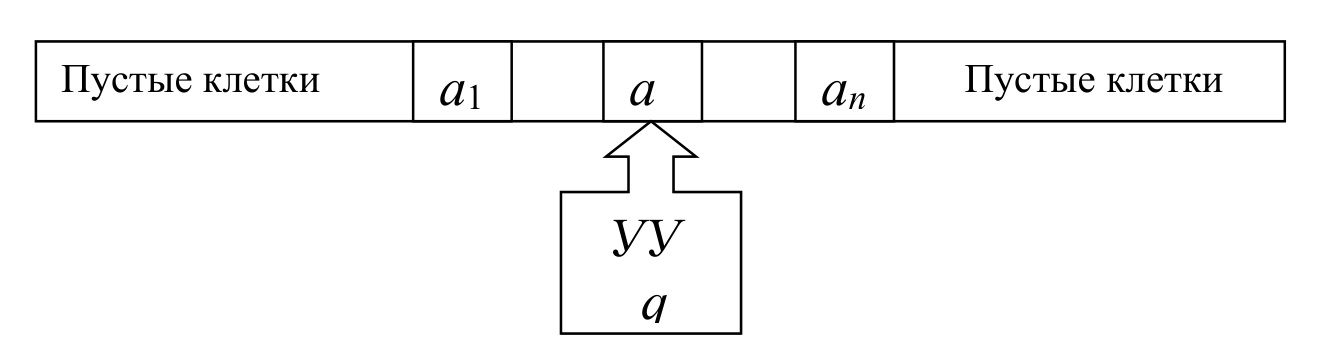
\includegraphics[scale=0.25]{графика/тьюринг.png}
\end{figure}

\begin{enumerate}
    \item Символы внешнего алфавита $\Sigma = \{0,1,\dots\}$ записываются в ячейки конечной ленты, которя называется \textbf{внешней памятью машины}, при необходимости в ячейки записывается символ *, который называется \textit{пустым}
    \item Символы внутреннего алфавита $Q=\{q_S,q_F,\dots\}$ обозначают состояния \textbf{управляющего устройства машины} (УУ) с \textbf{просматривающей головкой}, которая может перемещаться вдоль ленты и в каждый момент времени $t$ просматривать одну ячейку
    \item \textbf{Программа машины} $$\Pi = \{T(q,a:q\in Q \backslash \{q_F\} \land a \in \Sigma)\}$$ состоит из \textbf{команд} $T(q, a) = qa \to q'a'X$, которые в зависимости от состояния машины $q$ и символа $a$ в просматриваемой ячейке УУ заменяют в этой ячейке букву $a$ на букву $a'$, состояние $q$ на состояние $q'$ и в зависимости от значения $X \in \{R, L, S\}$ сдвигают просматривающую головку либо в соседнюю правую ячейку при $X = R$, либо в соседнюю левую ячейку $X = L$, либо оставляет головку на месте при $X = S$. При необходимости на ленте достраиваются справа или слева ячейки с пустым символом $*$
    \item Машина начинает работать в \textbf{начальном состоянии} $q_S$ и заканчивает работать в \textbf{заключительном} состоянии $q_F$
\end{enumerate}

Вход машины: слово $w \in \Sigma*$ на ленте машины $T$ в начальном состоянии $q_S$.

Выход машины: слово $s' \in \Sigma*$ на ленте машины $T$ в заключительном состоянии $q_F$.

Строго математически такие машины определяются следующим образом.

\subsection{Математическое описание машины Тьюринга}
\dftion \textbf{Машина Тьюринга} $T$ представляет собой алгебраическую систему $T = (\Sigma, Q, \delta, q_S, q_F)$, работающую в дискретные моменты времени $t=0,1,2\dots$ и состоящую из следующих частей:

\begin{itemize}
    \item Конечное множество $\Sigma=\{0,1\dots\}$ называется \textit{внешним алфавитом}
    \item Конечное множество $Q = \{q_S, q_F, \dots\}$ называется \textit{внутренним алфавитом}, элементы $Q$ называются \textit{состояниями машины}
    \item Отображение $\delta: Q \times \Sigma \to Q \times \Sigma \times \{R, L, S\}$, которое определяет список команд $T(q, a) = qa \to q'a'X$ --- символическое оюозначение образов $\delta(q, a) = (q', a', X)$ отображения $\delta$ для $q \in Q \backslash \{q_F\}, a \in \Sigma$ и $X \in \{R, L, S\}$, множество всех команд $\Pi = \{T(q, a): q \in Q \backslash \{q_F\} \land a \in Sigma\}$ называется \textit{программой машины}
    \item Состояние $q_S$ называется \textit{начальным} и означает начало работы машины
    \item Состояние $q_F$ называется \textit{заключительным} и означает завершение работы машины
\end{itemize}

Работа машины Тьюринга $T$ происходит под действием её команд и заключается в измений её \textit{конфигураций}, описывающих состояния ленты и управляющего устройства, а также положение головки относительно ячеек ленты: если лента находится в состоянии, которое описывается словом $\alpha a \beta$ над алфавитом $\Sigma$, и головка в состоянии $q$ просматривает на ленте ячейку с состоянием $a$, то соответствующая конфигурация $K$ машины $T$ описывается выражением $M=\alpha q a \beta$, которое называется \textbf{машинным словом}.

При этом $K$ называется \textbf{начальной конфигурацией}, если описывающее её машинное слово содержит символ начального состояния $q_S$, и \textbf{заключительной конфигурацией}, если описывающее её машинное слово содержит символ заключительного состояния $q_F$.

Программа указывает, что машина делает в каждый момент времени в зависимости от её настоящей конфигурации $K$:
\begin{itemize}
    \item Если $K$ --- заключительная конфигурация, то машина заканчивает работу
    \item Если K не является заключительной конфигурацией и описывается машинным словом $M=\alpha q a \beta$, то в программе $\Pi$ машина находит команду $T(q, a)$ с левой частью $qa$ и в зависимости от вида правой части такой команды $T(q,a)$ машина заменяет в просматриваемой ячейке букву $a$ на букву $a'$, состояние $q$ на состояние $q'$ и в зависимости от значения $X \in \{R, L, S\}$ сдвигают просматривающую головку либо в соседнюю правую ячейку при $X = R$, либо в соседнюю левую ячейку при $X = L$, либо оставляет головку на месте при $X = S$
\end{itemize}

Изменение конфигруаций $K_0, K_1, K_2, \dots$ машины $T$ под действием команд происходит в дискретные моменты времени $t = 0, 1, 2, \dots$ и описывается преобразованием соответствующих машинных слов $M_0, M_1, M_2, \dots$ по следующему правилу. За один шаг работы машины $T$ её машинное слово $M = \alpha q a \beta$ под действием команды $T(q ,a)$ преобразуется в новое машинное слово $M'$ по формулам:
\begin{itemize}
    \item если $T(q,a) = qa \to q'a'S$, то $M' = \alpha q' a' \beta$
    \item если $T(q, a) = qa \to q'a'R$ и $M = \alpha q a b \beta'$, то $M' = \alpha a'q'b\beta'$
    \item если $T(q,a) = qa \to q'a'R$ и $M=\alpha q a$, то $M' = \alpha a' q' *$
    \item если $T(q,a) = qa \to q'a'R$ и $M = \alpha q a$, то $M' = \alpha a' q' *$
    \item если $T(q, a) = qa \to q' a'L$ и $M=\alpha'bqa\beta$, то $M'=\alpha'q'ba'\beta$,
    \item если $T(q,a) =  qa \to q'a'L$ и $M = qa\beta$, то $M' = q'*a'\beta$
\end{itemize}

Символически такое одношаговое преобразование машинных слов обозначается $M \to^T M'$.

Если существует такая последовательность преобразований машинных слов $M_i \to^T M_{i+1}$ (где $i = 0,1,\dots,k-1$), для которой $M_0 = M$ и $M_k = M'$, то пишут $M \then^T M'$ и говорят, что машинное слово $M'$ получается из машинного слова $M$ с помощью машины $T$.

\dftion \textbf{Вход} (начало работы) машины: слово $w \in \Sigma*$ на ленте машины $T$ в начальном состоянии $q_S$.

\dftion \textbf{Выход} (завершение работы) машины: слово $w' \in \Sigma*$ на ленте машины $T$ в заключительном состоянии $q_F$.

В этом случае говорят, что машина $T$ \textbf{принимает} слово $w$ и выдаёт значение $w'=T(w)$. В результате машина $T$ определяет язык $L(T)\subset\Sigma*$, который состоит из всех принимаемых машиной $T$ слов.

\dftion Язык $L \subset \Sigma*$ \textbf{принимается} машиной Тьюринга, если $L=L(T)$ для некоторой машины Тьюринга $T$.

Таким образом, любая машина Тьюринга $T$ определяет частичную функцию $f$ из $\Sigma*$ в $\Sigma*$, область определения которой $D_f$ состоит из всех слов алфавита $\Sigma$, которые принимает машина $T$, и значения которой для слов $w \in D_f$ определяются по формуле: $f(w) = T(w)$.

\dftion Частичная фунция $f$ из $\Sigma*$ в $\Sigma*$ называется \textbf{вычислимой по Тьюрингу}, если она определяется некоторой машиной Тьюринга.

\underline{Пример}. Пусть машина Тьюринга $T$ имеет внешний алфавит $\Sigma=\{0,1\}$, внутренний алфавит $Q=\{q_S,q_F, q\}$ и программу $\Pi$, которая состоит из команд $q_S1\to q1R, q1\to q1R, q* \to q_F 1S$. Тогда слово $\alpha=11$ машиной $T$ перерабатывается в слово $\beta=111$, так как
$$ \underline{q_s1}1 \underset{(1)}\to^T 1\underline{q1} \underset{(2)}\to^T 11\underline{q*} \underset{(3)}\to^T 11\underline{q_F}1 ~ \text{и} ~ T(11) = 111. $$

Легко видеть, что любое слово $\alpha = 1^n$ над алфавитом $\Sigma=\{0, 1\}$ машиной $T$ перерабатывается в слово $\beta = \alpha 1 = 1^{n+1}$. Это означает, что машина $T$ к любому слову над алфавитом $A = \{1\}$ приписывает справа символ 1.

\dftion Частичная словарная функция $f:(\Sigma*)^n \to \Sigma*$ над алфавитом $\Sigma$ называется \textbf{вычислимой по Тьюрингу}, если существует машина Тьюринга $T$ с внешним алфавитом $\Sigma$, для которой при любых $w_1, \dots, w_n \in \Sigma*$ условие $(w_1, \dots, w_n) \in D_f$ равносильно тому, что машина $T$ применима к слову $\alpha = w_1 * \dots * w_n$ и результат $T(\alpha)$ переработки данной машиной $T$ такого слова равен значению функции $f(w_1,\dots,w_n)$.

\textbf{Основная теорема}.
Для любой частичной словарной функции $f: (\Sigma*)^n \to \Sigma*$ следующие условия эквивалентны:

\begin{enumerate}
    \item Функция $f$ вычислима по Тьюрингу
    \item Функция $f$ частично рекурсивна
    \item Функция $f$ нормально вычислима
\end{enumerate}

Такие вычислительные процедуры называются \textbf{алгоритмами}.

\section{Вычислимость: разрешимые и полуразрешимые языки}
\underline{Определение 1}. Язык $L$ называется \textit{разрешимым} (или \textit{рекурсивным}), если существует такая машина Тьюринга $T$, что для любого слова $w \in W$ выполняются условия:
\begin{itemize}
    \item если $w \in L$, то при входе $w$ машина $T$ попадает в заключительное состояние, останавливается и выдаёт значение $T(w) = 1$
    \item если $w \not \in L$, то при входе $w$ машина $T$ попадает в заключительное состояние, останавливаетс и выдаёт значение $T(w) = 0$
\end{itemize}

Такие машины соответствуют понятию <<алгоритма>> и применяются при решении \textit{распознавательных задач} типа <<да/нет>>.

Множество всех разрешимых языков будем обозначать $R$ (от Recursive).

\textbf{Свойства}: дополнения, конечные пересечения и конечные объединения разрешимыъх языков являются разрешимыми языками.

\textbf{Примеры разрешимых языков}.
\begin{itemize}
    \item Пустой язык
    \item Множество всех строк
    \item Конечные множества
    \item Множество чётных чисел
    \item Множество простых чисел
    \item Множество рациональных чисел, не превышающих $e$
    \item Множество всех чисел $n$, при которых в $\pi$ не меньше $n$ девяток подряд
\end{itemize}

\underline{Определение 2}. Язык $L$ называется \textit{полуразрешимым} или \textit{перечислимым}, если существует такая машина Тьюринга, что
\begin{equation}
    L = L(T) = \{w \in \Sigma* : T(w) = 1\},
\end{equation}
то есть при выходе $w \in L$ машина $T$ попадает в заключительное состояние, останавливается и выдаёт значение $T(w) = 1$, а при выходе $w \not \in L$\dots\dots\dots

\underline{Лемма}. Существуют неразрешимые языки, поскольку алгоритмов счётное число, а языков несчётное.

Аналогично можно доказать, что существуют языки, не являющиеся полуразрешимыми.

\underline{Основная теорема}. Существуют полуразрешимые неразрешимые языки, т. е. полуразрешимые языки, которые не могут быть разрешимы никакм алгоритмом, т. е. выполняется свойство $R \not \subset RE$.